\documentclass{article}

\usepackage{xurl}
\usepackage{amsmath, amsthm, amssymb, amsfonts}
\usepackage{thmtools}
\usepackage{graphicx}
\usepackage{setspace}
\usepackage{geometry}
\usepackage{float}
\usepackage{hyperref}
\usepackage[utf8]{inputenc}
\usepackage[english]{babel}
\usepackage{framed}
\usepackage[dvipsnames]{xcolor}
\usepackage{tcolorbox}
\usepackage{titlesec}
\usepackage{xcolor}
\usepackage{setspace}
\usepackage{fancyhdr}
\usepackage{orcidlink}

%| ----------------------------------------------------------------------------------------------------------------- |%

\newcommand{\HRule}[1]{\rule{\linewidth}{#1}}
\newcommand{\OpenDyslexic}[1]{
    {
        \defaultfontfeatures{Mapping=tex-text,Scale=MatchLowercase}
        \setmainfont{OpenDyslexic}
        \fontsize{24}{26}\selectfont\setstretch{0.5}
        #1
    }
}

%| ----------------------------------------------------------------------------------------------------------------- |%

\setcounter{secnumdepth}{4}
\titleformat{\paragraph}{\normalfont\normalsize\bfseries}{\theparagraph}{1em}{}
\titlespacing*{\paragraph}{0pt}{3.25ex plus 1ex minus .2ex}{1.5ex plus .2ex}

%| ----------------------------------------------------------------------------------------------------------------- |%

\setstretch{1.2}
\geometry{ textheight=9in, textwidth=5.5in, top=1in, headheight=12pt, headsep=25pt, footskip=30pt }

%| ----------------------------------------------------------------------------------------------------------------- |%

\title{ 
    \normalsize 
    \textsc{} \\
    [2.0cm]
    \HRule{1.5pt} \\
    \LARGE \textbf{
        \uppercase{Educational sciences}
        \HRule{2.0pt} \\ 
        [0.6cm] 
        \LARGE{Final Essay} 
        \vspace*{10\baselineskip}
    }
}
\date{\today}
\author{
    \textbf{Tygo van den Hurk}\,\orcidlink{0009-0003-4182-5076}\textit{(1705709)}
}

%| ----------------------------------------------------------------------------------------------------------------- |%

\begin{document}   

    %| ------------------------------------------------------------------------------------------------------------- |%
    %|                                                  Cover Page                                                   |%
    %| ------------------------------------------------------------------------------------------------------------- |%
    
    \maketitle
    \thispagestyle{empty}
    \newpage
    
    %| ------------------------------------------------------------------------------------------------------------- |%
    %|                                               Table of Contents                                               |%
    %| ------------------------------------------------------------------------------------------------------------- |%
    
    \renewcommand{\contentsname}{Inhoudsopgave}
    \tableofcontents
    \thispagestyle{empty}
    \newpage

    %| ------------------------------------------------------------------------------------------------------------- |%
    %|                                           Persoonlijke achterground                                           |%
    %| ------------------------------------------------------------------------------------------------------------- |%

    \section{Persoonlijke achtergrond}
        \textbf{Persoonlijke achtergrond: Schets hier jouw onderwijscarrière tot nu toe en hoe je die wenst voort te zetten. Gebruik de zelfportret opdracht uit bijeenkomst 1. Welke ervaringen heb je gehad als leerling en als docent? Wat is jouw toekomstperspectief? Denk je dat je docent gaat worden/blijft? Waarom wel/niet? En binnen wat voor soort omstandigheden/welke doelgroep/welk vak?}
        
        \subsection{Achtergrond}
            Als ik mijn achtergrond kort zou moeten beschrijven, dan zou dat ook de manier zijn hoe ik hem zou moeten beschrijven, kort. Ik heb in mijn jaren niet veel op genomen actief. In mijn mening, ben ik door de basis- en middelbare school heen gevlogen. zonder mijn heresenen aan te hoeven zetten. Daar gebeurde op beide niet veel. De stof was makkelijk, en ik heb als kind niet veel opgelet wat de leeraar, klasgenoten, of zelfs ik deed. Ik was voornamelijk bezig met hoe ik stiekem kon strips kon maken terwijl ik aan het "rekenen" was. Het is pas nu, als ik reflecteer dat ik over wat ik nog kan herrinier kan na gaan waarom mensen dingen deden.

            \subsubsection{Leerling's Perspectief}
                Zoals hierboven vermeld was ik niet perse een goede student. Heel plat gezegd was ik gewoon slimmer dan dat je voor de stof hoefte te zijn en kon ik mijn weg er doorheen faken, of met minimale moeite doen. Dat maakte mij snel afgeleid en bezig met dingen bezig die ik intresant vond.
                \bigskip
                \noindent Er zijn wel dingen die ik me kan herineren waar ik een mening over heb. In groep 6 had ik een leeraar die kinderen deed pesten om ze te laten gedragen hoe hij wilde. Als ik was weg gedroomd deed hij altijd luid "Ik zat even niet op te leten, kwam met mijn vingers tussen de castagnetten..." een liedje van Bertus Staigerpaip te zingen, zodat iedereeen dat kon horen of dat zette hij dan aan op youtube. Een andere peste hij voor zijn kleine blaas omdat hij te vaak naar het toilet moest. Hij at krijtjes om te schuimbekke zodat ie ze je kon laten schrikken. Een nare man. Ik zou zeggen, dat is hoe het niet moet.
                \bigskip
                \noindent Jaar daar na, in groep 7, kreeg ik juf Ellie en juf Inge. Dat was dan weer een voorbeeld over hoe je het wel moest doen. Hun waren leeraren die kinderen begrepen en het beste er uit wilde halen. In plaats van mij te pesten omdat ik snel afgeleid was waren ze er juist voor om mijn concentratie op te bouwen. Ze lieten me steeds langer concentren. Eerst maar 5 minuten aan een stuk. Dan moest ik 5 minuten rekenen. Endaarna mocht ik 5 minuten tekenen. Ik vond dat best eerlijk 50/50. Dan bouwede ze het langzaam op naar 20 minuten rekenen. 5 minuten tekenen. Dit heet progressive concentration training heb ik zojuist op gezocht en dit, is in mijn mening wel een manier hoe je met kinderen moet omgaan, hoe je leeraar kan zijn.

            \subsubsection{Leeraar's Perspectief}
                Ik heb nog niet veel ervaring als een leeraar. Ik heb hockey les gegeven daar had ik veel plezier aan. Het probleem is dat ik alleen me snel in chaos liet trekken. Ik ben zelf van nature veel random, chaotisch, en impulsief. Dat is de ADHD, maar dat maakte het niet makkelijker om met 13 kleine kinderen te moeten dealen. Dus dat is iets waar ik aan het werken ben.
                \bigskip
                \noindent Ik heb ook stof uit gelegd aan mede leerlingen voordat ik op uni ook zelf begon te struggelen. Hoewel dat niet altijd goed ging, en het kwartje niet altijd meteen viel merkte ik wel dat de efectiviteit wel flink verschilde per persoon. Ik denk dat dit is omdat de manier hoe ik begreep niet altijd logisch was voor andere en andersom. Dat is natuurlijk omdat ieder mens anders denkt en een ander brein heeft. Maar dat bracht mij wel op een idee voor hoe ik dit in de toekomst wil zien.

        \subsection{Toekomst Visie}
            Dat brengt mij op mijn visie voor de toekomst. Ik had, en heb nog steeds struggles met mijn brein. Mijn brein is wat je heel "bijzonder" zou noemen. Met ADHD, Dyslextie, en wat op dit moment onderzocht word waarschijnlijk autisme. Dat betekend dat mijn brein op een andere manier is opgebouwd, denkt, functioneer, groeit, verwerkt, of stof op neemt\cite{neurodivergent}. 
            \bigskip
            \noindent Dat is niet perse slecht, soms is dit een super sterke kant. Denk aan bijvoorbeeld een kenmerk van ADHD genaamd "hyperfocus"\cite{hyperfocus} veel van ons die ADHD hebben beschikken hierover. Dit is een soort focus waar je in kan stappen — technisch gezien val je hier meer in — waarin je de hele wereld vergeet en je brein alleen maar die activiteit die je aan het doen bent kan ademen. Er zijn vele dagen — zeker nu dat ik op mezelf woon — dat ik lunch, en avondeten vergeet. Dat is niet mijn bedoeling, maar calculus klikte en kwam in de flow en voor ik het wist was het 10 uur s'avonds.
            \bigskip
            \noindent Mijn punt dat ik wilde maken hier is omdat iedereen anders is, iedereen ook andere behoefte heeft. Mensen met ADHD, autisme, dyslextie, en zelf queerness hebben gewoon een andere brein dan neurotypische mensen\cite{ADHD-Neurobiologie}\cite{Autisme}\cite{Dyslextie-breinen}\cite{LGBT-vs-CISHET-breinen}. Daarmee hebben zij ook andere behoefte\cite{ADHD-Bijkomende-problematiek}\cite{ADHD-behoeftes}. Mijn toekomst visie is dat neurodivergent breinen ook het onderwijs krijgen dat ze nodig hebben en dat ondanks dat ze andere brein structuren hebben ze niet perse tweede rangs onderwijs hoeven te hebben. Maar hier vertel ik in de sectie "Mijn Ideal Les" meer over.

        \subsection{Terug koppeling on mijn Zelf-Portret}
            Om terug te komen op mijn zelf potret. Ik weet nog steeds niet of ik leeraar wil worden. Wat ik wel weet is dat als ik leeraar word. Ik graag wil zorgen dat het onderwijs inclusiever word. Er kan nog zo veel gedaan worden om het onderwijs beter te maken voor iedereen. En of ik voor de klas wil staan en op die manier die verandering wil maken, dat weet ik nog niet. Maar dat die verandering op een bepaalde manier moet komen — one way, or another — dat weet ik wel. Dat voel ik.

    \newpage
    
    %| ------------------------------------------------------------------------------------------------------------- |%
    %|                                              Taak van de Docent                                               |%
    %| ------------------------------------------------------------------------------------------------------------- |%

    \section{Taak van de docent}
        \textbf{Taak van de docent: Wat zouden voor jou de belangrijkste taken van een docent zijn? (denk bijv. aan: voorbereiden vervolgopleiding, enthousiasmeren, opleiden als goede burger, algemene basiskennis aanleren, sociaal-emotionele ontwikkeling, het 'leren leren', 21e eeuwse vaardigheden aanleren etc). Benoem ze niet allemaal, maar bedenk welke twee jij het belangrijkste vindt en beschrijf waarom die twee voor jou centraal staan.}
        \bigskip
        \noindent Naar mijn mening is de rol van een docent veelzijdig, maar ik beschouw twee rollen als bijzonder cruciaal. For starters vind ik Enthousiasmeren het aller belangrijkst en met Promotor van Sociaal-Emotionele Ontwikkeling op de tweede plaats.
        
        \subsection{Enthousiasmeren}
            Het belangrijkste uit dit lijstje vind ik \textit{Enthousiasmeren}, by far. Als leerling werd ik niet vaak enthousist gemaakt over de stof en had mede daarom moeite met het beginnen aan de stof, en blijven werken aan de stof. Als leerlingen enthousiast worden gemaakt over de stof is het niet alleen makkelijker om ze aan de stof te laten beginnen, het is ook makkelijker voor hun om er mee bezig te blijven. Dit is omdat leerlingen die enthousiast zijn over een onderwerp intrinsieke motivatie aanmaken.\cite{enthusiasm-creates-motivation}
            \bigskip
            \noindent Hoewel zowel intrinsieke als extrinsieke motivatie resultaten positivief beinvloeden, bleek dat voor de prestaties van mensen intrinsieke motivatie het belangrijkste is.\cite{intrinsic-motivation-is-more-important} Niet alleen is het makkelijker dat leerlingen uit zich zelf aan de stof beginnen, en bezig blijven met de stof. Daar boven op maakt het dat ze actief bezig zijn met de stof. Ze nemen het veel sneller en dieper op. Als leerlingen leren omdat ze extrinsiek gemotiveerd zijn nemen ze de stof veel oppervlakkiger op\cite{extrinsic-motivation-results-in-supperfical-learning}. Een ander aspect van leerlingen die extrinsiek gemotiveerd zijn is dat omdat ze het willen leren ze naar je toe komen voor hulp en begeleiding. Hierdoor krijg je dat de sfeer zich automatisch op steld als samen-boven. Wat door zowel leerlingen als leeraren werd gezien als de ideale combinatie. Niet alleen vinden beide dit het beste, ook bleek dat samen-boven leid tot betere prestaties.\cite{samen-boven-leads-to-better-results} Daarom vind ik intrinsieke motivatie veel belangrijker dan extrinsieke motivatie en wil ik die zoveel mogelijk opwekken. 
        
        \subsection{Promotor van Sociaal-Emotionele Ontwikkeling}
            Als tweede vind ik sociaal-emotioneel leren super belangrijk. Ik ben van mening dat voor kinderen — en sommige volwassenen — het net zo belangrijk is dat ze Sociaal en Emotioneel capabel zijn als dat ze weten hoe je een keer sommetje maakt. Het feit dat sommige volwassenen nog steeds niet weten hoe je je in sociale momenten je op moet stellen. Of dat ze nog steeds niet uitgevogeld hebben je met je emoties om moet gaan absurd.
            \bigskip
            \noindent 1 op de 10 mensen van de Nederlandse bevolking heeft psycholoog, psychiater of psychotherapeut bezocht, dat is 10\%.\cite{1-in-10-pygy} Ik ben van mening dat emotionele volwassenheid en capaciteit zeer in waarde word onderschat. Emotioneel volwassen worden hoort minstens even goed bij de opleiding van hoe je later een succesvolle deelnemer word in de maatschapij.
            \bigskip
            \noindent Emoties, hoe je hier mee om moet gaan is niet makkelijk voor iedereen. Sommige mensen hebben ouders die het zelf niet weten. Hoe kunnen die kinderen het dan aan leren? Daarom denk ik dat dit een must have skill is voor iedereen die met kinderen om moet gaan. Het is namelijk zo dat iemand emotionele staat extreem belangrijk is voor, hun welzijn, motivatie, en uiteraards prestaties. 
            \bigskip
            \noindent Een ander groot probleem dat je hier mee helpt is een versie van generational trauma. Kinderen die niet leren omgaan met hun emoties, kunnen hun kinderen niet leren omgaan met hun emoties. Deze kinderen kunnen zelf als ouders ook niet hun kinderen leren omgaan met emoties enz. Daarom is het naar mijn mening net zo belangrijk als rekenen dat kinderen leren hoe ze met emoties om moeten gaan.
            \bigskip
            \noindent Verder is het voor kinderen heel belangrijk om sociale contacten te hebben. Kinderen moeten sociale banden hebben voor hun ontwikkeling.\cite{social-isolation-affect-a-childs-mental-health-and-development} Het missen van sociale connecties is niet alleen slecht voor hun ontwikkeling. Het zorgt er ook voor dat ze later in het leven minder vrienden hebben. Wat niet goed is voor hun welzijn in de long term. Dit is ook een eis volgens motivatietheorie. Waardoor ik vind dat het hoog op de prioriteiten van elke leeraar moet staan.

    \newpage
    
    %| ------------------------------------------------------------------------------------------------------------- |%
    %|                                               Mijn Ideale Les                                                 |%
    %| ------------------------------------------------------------------------------------------------------------- |%
    
    \section{Mijn Ideale Les}
        \textbf{De ideale les: Hoe ziet een ideale les er volgens jou uit? Bespreek hier welke leer activiteiten de leerlingen uitvoeren en hoe je die als docent wilt aansturen, inclusief hoe je je daarbij opstelt in termen van interpersoonlijk gedrag. Ga ook in op de tijd, leeromgeving, materialen en groeperingsvormen (zie curriculair spinnenweb). Onderbouw deze ideale les: waarom is dit voor jou een ideale les? Gebruik daarvoor de theorie van Onderwijskunde 1 (wat je hebt geleerd over de neuropsychologie, motivatie en leer theorie) en verwijs ook naar deze theorie. Onderbouw ook met je eigen ervaringen. Wat van wat jij zelf hebt meegemaakt maakt dat je dit als een ideale les ziet en waarom? Je kunt deze les opzetten als een doelsysteem, met de onderbouwingen gekoppeld aan de les onderdelen.}
        \bigskip
        \noindent Deze sectie ga ik iets anders doen dan dat de opdracht is, maar dit doe ik expres, stay with me. Zover als ik begreep van de opdracht moest je je ideale les beschrijven. Één les. Sinds dat mijn toekomst visie iets breder is dan dat de typische leerling een mooie les mag hebben etcetra. Ga ik deze opdracht ook iets breder maken dat dat nodig is. En kies ik er voor om dieper in te gaan op stof die ik voor deze opdracht behandeld heb. 
        \bigskip
        \noindent Maar vrees niet, ik kom uiteindelijk waar ik zijn moet. Dus uiteindelijk krijg je waar je om vraagt. We nemen alleen even een in ADHD-fasion wat men een "flinke detour" zou noemen.
        
        \subsection{Theorie over het Les geven aan Neurodivergenten-Leerlingen}
            Neurodivergeten leerlingen hebben andere struggles dan neurotypical leerlingen, dat heb ik inmiddels al vijf keer gezegd. Maar wat zijn deze struggles, en wat zijn strategien die we toe kunnen passen om deze struggles te verminderen? De ene manier om deze vraag te beandwoorden is door het eerst op te breken in de verschillende soorten van neurodivergentie\cite{neurodivergent-types}. 
            
            \subsubsection{ADHD}
                \paragraph{ADHD: Struggles}\\
                    Hoewel ADHD veel symptomen en struggles heeft gaan we het hier vandaag alleen hebben over de struggles die van toepassing zijn op de les omgeving:
                    \begin{itemize}
                        \item \textbf{Wanorde en problemen met prioriteren}: 
                            Mensen met ADHD kunnen eigenlijk alleen taken doen die hun stimuleren. Als de taak dat niet is, is het bijna onmogelijk om je te concentrenen op deze taak. Een taak is snel stimulerend als het urgent is. Dit is omdat de taak leid tot het loslaten van adrealine. Doordat niet stimulerenende taken eigenlijk pas mogelijk worden zodra ze urgent worden zijn belangrijken taken vaak niet aan de orde, ze zijn namelijke nog niet urgent. Pas wanneer ze urgent worden, worden ze stimulerened genoeg om te kunnen doen. Hierdoor is er vaak een mismatch met wat belangrijk is en met wat urgent is, vandaar de problemen met prioriteren.\emph{\hyperlink{https://www.youtube.com/watch?v=5xbD9t8cM4M}{Deze video}}\cite{ADHD-video-prioriteiten} legt heel goed uit waarom dit zo moeilijk is.
                        \item \textbf{Slechte tijdmanagementvaardigheden}: 
                            omdat mensen met ADHD vaak zitten te wachten — zo voelen niet-stimulerende-taken vaak namelijk -, of juist zitten te hyperfocusen omdat iets wel stimulerened is en de tijd voorbij vliegt. Verschilt de perceptie in hoe snel tijd gaat veel op een dag. Hierdoor is het lastig voor mensen met ADHD om de tijd bij te houden. Daardoor hebben ze vaak een slechte time management. 
                        \item \textbf{Problemen met het concentreren op een taak}: 
                            als een taak niet stimulerend is is het bijna onmogelijk om je te kunnen concentreren op deze taak. Dit is omdat je brein meer stimulatie en dopamine nodig heeft om te kunnen functioneren. Hierdoor raak je snel afgeleid sinds je automatisch met taken die je wel stimuleren. Als een soort van junkie trekt je brein naar dingen die wel de stimulatie geven die het nodig heeft.
                        \item \textbf{Moeite met multitasking}: 
                            ieder brein heeft een bepaalde hoeveelheid werk geheugen. Dit is de hoeveelheid dingen die je in je hoofd kan houden. Bij mensen met ADHD is deze hoeveelheid lager. Dat betekend dat mensen met ADHD minder dingen te gelijker tijd kunnen herinneren en daarmee word multitasken moeilijk dan wel ommogelijk. \emph{\hyperlink{https://www.youtube.com/watch?v=HszXKZO_H18&ab_channel=HowtoADHD}{Deze video}}\cite{ADHD-video-working-memory} legt het heel goed uit
                        \item \textbf{Overmatige activiteit of rusteloosheid}: 
                            omdat mensen met ADHD graag bezig zijn en gestimuleerd worden is het lastig voor ons om soms stil te zitten en rust te nemen.
                        \item \textbf{Slechte planning}: 
                            dit is lastig voor ieder tiener brein, dat weet iedereen. Het probleem ligt alleen omdat mensen met ADHD niet snel kijken naar de toekomst (dit is namelijk niet urgent/stimulerend genoeg) hebben ze nooit de skill ontwikkeld om in de toekomst te kijken, en daarvoor te plannen. 
                        \item \textbf{Problemen met het afronden van taken}: 
                            als taken niet stimuleren genoeg zijn kan het zijn dat het dopamine potje opraakt en het brein ergens anders heen moet om dopamine te halen. Hierdoor kunnen mensen met ADHD soms moeilijk taken afroden.
                        \item \textbf{Emotionele regulatie}: 
                            de skill om emoties te behandelen en terug te komen naar de default state is lastiger voor mensen met ADHD. Dit uit zich in:
                            \begin{itemize}
                                \item intensere emoties
                                \item blijven hangen in die intense emoties
                                \item moeite met het omgaan met stress
                                \item snel voelen van emoties (die vervolgens heel intense zijn). 
                                \item Rejection Sensitivity, meer hierover kun je \hyperlink{https://www.youtube.com/watch?v=ZQ44ynEjsHQ&ab_channel=KatiMorton}{\emph{hier}}\cite{ADHD-video-rejection-sensitivity} zien, of \hyperlink{https://my.clevelandclinic.org/health/diseases/24099-rejection-sensitive-dysphoria-rsd}{\emph{hier}} lezen\cite{ADHD-rejection-sensitivity}.
                            \end{itemize}
                \end{itemize}
                \bigskip
                \noindent\paragraph{ADHD: Sterktes}\\
                    Gelukkig heeft ADHD ook een hoop sterkte punten. We gaan wel weer alleen in op de sterkte punten die relevant zouden kunnen zijn voor onze hypotetische les die we dadelijk gaan ontwerpen.
                    \begin{itemize}
                        \item \textbf{Hyperfocus}:
                            als je je leerlingen engaged en gestimuleerd kan krijgen is het mogelijk ze in hyper focus te krijgen. Als een leeraar leert hoe hij dit in diens leerlingen kan oproepen kan dat een goed sterkte punt zijn en leiden tot goede resultaten.

                        \item \textbf{ADHD Hardnekkigheid}:
                            mensen met ADHD zijn vaak veel vol houdender dan hun neurotypische counterparts. Dit komt omdat ze vaak meer moeite moeten doen om de zelfde taak te voltooien. Hierdoor geven mensen met ADHD vaak minder snel op, ze zijn namelijk gewend dat het niet meteen lukt.\cite{ADHD-resilience}
                        \item \textbf{Sociaal}: 
                            mensen met ADHD zijn over het algemeen veel socialer dan Neurotypische mensen. 
                        \item \textbf{Creatief}: 
                            dit is waarschijnlijk het meest bekende voordeel. Mensen met ADHD zijn vaak veel creatiever dan mensen zonder.\cite{ADHD-creativity}
                        \item \textbf{Visuele denkers}: 
                        mensen met ADHD denken veel visueler
                    \end{itemize}
                \bigskip
                \noindent\paragraph{ADHD: Leer tips}\\
                enkele tips die ik gevonden heb bij het les geven van mensen met ADHD zijn:
                \begin{itemize}
                    \item \textbf{Duidelijke Instructies Geven}: 
                        \textit{Bied duidelijke, stapsgewijze instructies en herhaal of herschrijf ze indien nodig}. Visuele hulpmiddelen en schriftelijke instructies kunnen nuttig zijn\cite{ADHD-visual}. ADHD'ers leren vaak met hun rechter brein. Hierdoor zijn ze veel visueler en leren ze beter als ze het zien of doen over het horen. Een ander voorbeeld is omdat mensen met ADHD een kleinere hoeveelheid werk geheugen hebben kan het zijn dat ze het nodig hebben om dingen opnieuw te kunnen lezen. Ik zal een voorbeeld geven waarin dit terug komt. 
                        \smallskip
                        Laten we zeggen dat een persoon zonder ADHD 4 dingen tegelijkertijd kan onthouden, en iemand met ADHD maar 3. Als je dan een vraag zou stellen aan beide leerlingen neem je een plek in beslag in dit werk geheugen. De niet-ADHD'er heeft er nog 3 over en de ADHD'er nog maar 2. Geef ze dan 3 mogelijke andwoorden op deze vraag en je hebt een probleem. Het hoofd van de normale leerling zit vol (1 vraag plus 3 andwoorden is 4, het maximale wat hij kan onthouden). Maar de ADHD leerling? Die is inmiddels de vraag vergeten. Je gaf 'm namelijk een vierde ding om te onthouden terwijl die er maar physiek 3 kan onthouden. Dit is wanneer de mogelijkheid om terug te kunnen lezen belangrijk kan zijn voor ADHD leerlingen.\cite{ADHD-video-working-memory}
                    \item \textbf{Visuele Ondersteuning Gebruiken}: 
                        \textit{Geef visuele schema's, grafieken en diagrammen}. Dit brengt ons terug op punt 1. Omdat ze visuele leerlingen zijn is het vaak handing om: 
                        \begin{itemize}
                            \item \textbf{Belangrijke dingen te kleuren en te markeren}. 
                                Dit help visueel de belangrijkste dingen uit elkaar te houden.
                            \item \textbf{oudere kinderen te leren hoe ze informatie kunnen visualieseren in diagramen}. 
                                Neem een voorbeeld aan een mind map. Deze heb ik persoonlijk altijd een investeering gevonden. Handig, maar wel tijd consumerend. Jongeren kinderen kun je laten teken wat ze aan het leren zijn. Op deze manier moeten ze de tijd en moeite nemen om het visueel voor te stellen. 
                        \end{itemize}
                        Deze goede voorbeelden kwamen van \emph{\hyperlink{https://www.additudemag.com/visual-learner-homework-help/}{additudemag.com}}. Je kan precieze link vinden in the references onder nummer \cite{ADHD-visual}.
                    \item \textbf{Taken Opsplitsen in Kleinere Stappen}: 
                        \textit{Verdeel complexe taken in kleinere, beheersbare stappen om overweldiging te voorkomen}. Omdat het werkgeheugen minder is, is het belangrijk dat je helpt met het eerst opslitsen van het probleem. Hierdoor raakt het hoofd van mensen met ADHD minder vol, en voorkom je een overload. Dit herkent iedereen wel. Dit is wanneer het je allemaal even te veel word en je brein het niet meer doet. Er zijn namelijk te veel dingen die je moet doen en je weet niet meer waar je mee moet beginnen. Deze drempel ligt bij mensen met ADHD lager. Daarom is het belangrijk dat je ze helpt met hoe ze dit zelf kunnen doen.
                        \smallskip
                        Een andere goede suggestie die gemaakt werd door \emph{\hyperlink{https://www.additudemag.com/visual-learner-homework-help/}{additudemag.com}} (zie reference \cite{ADHD-visual}) was om een \textit{Plan-of-Attack} te maken. Gezien het soms moeilijk kan zijn voor ons alle dingen op een rijtje te kunnen zetten. \textit{bullet list} zijn ook een super goede om toe te passen. Op deze manier kan je snel terug kijken of je niet iets vergeten bent.
                    \item \textbf{Een Zintuigvriendelijke Omgeving Creëren}: 
                        \textit{Creëer een comfortabele klasomgeving door rekening te houden met zintuiglijke gevoeligheden}. Bied zintuiglijke hulpmiddelen of ruimtes voor zelfregulering. Mensen met ADHD kunnen sneller over, of onder prikkeld worden. Het is belangrijk om de juiste hoeveelheid prikkels te bieden aan het brein en dit regelmatig te houden. Hoe ik dit bijvoorbeeld doe is het zelfde nummer op repeat te houden. Omdat dit je brein stimuleerd maar er toch ritme in zit houd je toch een soort van rust in je hoofd. Omdat het het zelfde nummer is word het heel voorspelbaar, en voor mij heel prettig.
                    \item \textbf{Regelmatig Feedback Geven}: 
                        \textit{Geef specifieke, constructieve feedback en lof om positief gedrag en prestaties te versterken}. Mensen met ADHD hebben behoefte aan snelle feedback. Het prettigste is om meteen feedback te krijgen of iets goed of fout was. Hierdoor krijg je meteen de dopamine die ons brein vereist om verder te gaan. Als we te lang moeten wachten kan dit leiden tot een concentratie, of motivatie problemen. Het probleem is namelijk niet stimulerend genoeg.
                \end{itemize}
            
            \subsubsection{Autisme}
                Autisme en ADHD gaan bijna hand in hand. 50\% tot 70\% van de mensen met autisme heeft ook ADHD\cite{ADHD-en-autisme-overlap}. Dit leid er dan ook toe dat beide zelfde zwaktes en sterke punten hebben.\\
                \noindent\paragraph{Autisme: Struggles}\\
                    We gaan wederom de zwakke kanten die niet relevant zijn voor het onderwijs weg laten voor de lengte. Dit mag dan wel een passie essay zijn maar we gaan al richting de 10 pagina's en ik ben nog lang niet klaar.
                    \begin{itemize}
                        \item \textbf{social anxity}: 
                            mensen met autisme hebben vaak moeite, vinden het eng om met mensen contact te maken. Persoonlijk denk ik niet dat dit een ding is dat autisme veroorzaakt maar omdat iemand met autisme vaak niet begrepen word door leeftijds genoten, en misschien zelf leeftijds genoten niet begrijpt word er een soort weerstand opgebouwd met interacties met leeftijds genoten. Want als het eerst niet goed ging, waarom zou het dan nu wel goed gaan?
                            \smallskip
                            Ik bedoel hier niet mee dat het even makkelijk is voor iemand met autisme als iemand zonder om een connectie te leggen. Want gezien je letterlijk op een andere manier je brein hebt opgebouwd is dit zeker niet het geval. Maar ik hoop door het onderwijs beter te maken voor mensen met autisme dat dit in de toekomst te minimaliseren. Het zal namelijk niet 100\% gelijk worden. Maar dat hoeft ook kan ook niet, en dat hoeft ook niet. Zolang als het maar beter, en makkelijker word.
                        \item \textbf{Emotionele regulatie}: 
                            vergelijkbaar met ADHD hebben mensen met autisme last van het reguleren van hun emoties. Dit maakt hun emoties, intenser en langer duurend dan hun neurotypische counterparts. Dit uit zich dan ook in verschillende kenmerken:
                            \begin{itemize}
                                \item druk maken om "niks"
                                \item obsessive compulsive behaviour (OCD)
                                \item meltdowns
                                \item phobias
                            \end{itemize}
                            om dit te voorkomen leerd het brein dingen aan om de emoties te voorkomen in plaats van te leren dealen met deze emoties. Voorbeelden hiervan zijn:
                            \begin{itemize}
                                \item hyper-vigilance, of “shell shocked” lijken
                                \item vermijdend gedrag
                                \item routines en weerstand aan veranderingen
                                \item controlerend gedrag
                                \item of in opstand komen tegen gezag
                            \end{itemize}
                        \item \textbf{shut downs}\cite{autisme-shutdowns}: Dit gebeurd wanneer iemand met autisme overloaded raakt.
                    \end{itemize}
                \bigskip
                \noindent\paragraph{Autisme: Sterktes}
                    \begin{itemize}
                        \item \textbf{Focused leren}\cite{autisme-upsides}: 
                            vergelijkbaar met ADHD's hyperfocus kan iemand met autisme de wereld kompleet vergeten en opgaan in waar ze mee bezig zijn.
                        \item \textbf{creativiteit en unique perspecitiven}\cite{autisme-upsides}:
                            Kinderen met autisme hebben vaak een unique blik op iets. Gezien hun brein anders is opgebouwd, en anders informatie verwerkt krijg je natuurlijk ook een andere output!
                        \item \textbf{empathie}\cite{autisme-upsides}: 
                            in tegen stelling tot wat andere denken hebben mensen met autisme meer empathie dan hun neurotypische tegenliggers. Deze mythe komt doordat het moeilijk is om neurotypische mensen om de informatie uit de persoon met autisme te halen.
                        \item \textbf{beter geheugen}\cite{autisme-upsides}: 
                            mensen met autisme hebben vaak een heel goed geheugen. Zeker voor details of patronen. Dit is een van de sterkste kanten van iemand met autisme.
                        \item \textbf{oog voor detail}\cite{autisme-upsides}: 
                            niet alleen kunnen mensen met autisme goed details onthouden, het spotten van details gaat ze heel makkelijk af. Ze zien deze veel beter dan hun neurotypische tegenliggers.
                        \item \textbf{Harnekkigheid}\cite{autisme-upsides}:
                            net zoals ADHD'ers zijn mensen met ADHD hardnekkig en geven ze niet zomaar op. Zekere niet als ze een passie hebben voor iets en ze in hyperfocus gaan.
                    \end{itemize}                    
                 \bigskip
                 \noindent\paragraph{Autisme: Les tips}
                     \begin{itemize}
                         \item \textbf{Structuur en Routine}\cite{autisme-teaching-them}:
                             Het is voor mensen mte autisme heel belangrijk om structuur en routine te hebben. Dit houd ze gefocusd op de taak en zorgt dat ze zich geen zorgen hoeven te maken over kleinen dingen. Een voorbeeld is om na ieder vak kinderen hun spullen op te laten ruimen. Dit geeft dan mentaal het einde van het onderwerp aan. Dit houd het klaslokaal schoon, en structuur in ons hoofd.
                         \item \textbf{Vermijd stimulerende factoren}\cite{autisme-teaching-them}:
                             Om te voorkoment dat mensen met autisme over prikkeld raken is het belangrijk om te zorgen dat de stimulatie tot een minimum getrokken word.
                         \item \textbf{zeg zo min mogelijk en schrijf dingen op}\cite{autisme-teaching-them}:
                             mensen met autisme zijn visuele leerlingen\cite{autisme-visual}. Dus net zoals met ADHD helpt het om:
                                 \begin{itemize}
                                     \item duidelijke, stapsgewijze instructies te geven. Herhaal of herschrijf ze indien nodig
                                     \item bied visuele hulpmiddelen zoals highlights/markeren, diagramen 
                                     \item geef schriftelijke instructies in plaats van een heel verhaal te vertellen
                                     \item Laat oudere kinderen te leren hoe ze informatie kunnen visualieseren in diagramen.
                                     \item laat jongeren kinderen kun je laten teken wat ze aan het leren zijn. 
                             \end{itemize}
                             zie de hierboven les tips voor ADHD voor meer informatie.
                         \item \textbf{beprek keuzes}\cite{autisme-teaching-them}:
                             Omdat mensen met autisme focusen op details, en heel analytisch denken kan het zijn dat simple keuzes heel moeilijk kunnen zijn. Als je ze bijvoorbeeld een kleur laat kiezen beperk de opties dan tot 3 verschillende kleuren.
                         \item \textbf{creer een-op-een sociale interacties}\cite{autisme-teaching-them}:
                             Door kinderen met autisme de kans te geven om een op een met 
                     \end{itemize}

            \subsubsection{Dyslextia}
                \paragraph{Dyslextia: Struggles}\\
                    \begin{itemize}
                        \item \textbf{Leesvaardigheden}\cite{dyslextia-struggles-and-superpowers}:
                            Dit is waaschijnlijk de meest bekende problemen die mensen met Dyslextia hebben. 
                        \item \textbf{Schrijfvaardigheden}:
                            Dit is waaschijnlijk het andere meest bekende probleem die mensen met Dyslextia hebben.
                        \item \textbf{Het omkeren van letters en cijfers tijdens het lezen (bijvoorbeeld "zag" lezen als "was")}\cite{dyslextia-struggles-and-superpowers}:
                            Een veel voorkomend probleem is het omkeren van letters zoals 'b' en 'd', of 'p' en 'q'. Gezien dit de zelfde letter is maar dan geroteerd, of gespiegeld.
                        \item \textbf{Notities maken in lessen en lezingen}\cite{dyslextia-struggles-and-superpowers}:
                            Gezien het Lezen en Schrijfven al lastig is, is het voor dyslexten bijna onmogelijk om zowel te lezen, schrijven en luisteren te gelijker tijd.
                        \item \textbf{Sequentiële instructies volgen}\cite{dyslextia-struggles-and-superpowers}:
                            Dit heeft wederom te maken met werk geheugen. Mensen met dyslextie hebben er niet perse minder van zoals met ADHD. Maar het is gebleken dat er verschillende soorten werkgeheugen zijn\cite{dyslextia-different-types-of-memory}. Voornamelijk visueel en auditorisch. (theoretisch zijn er meer vormen. Voor elk zintuig een). Om dingen het beste te onthouden moet men zo veel mogelijk van deze te gelijker tijd gebruiken. Dit geeft je de grootste kans iets te herinneren. Hier is het probleem, mensen met dyslextie hebben een dramatisch slechter auditorisch geheugen. Wat dus betekend dat je daar minder op kan leunen, en daarom alleen maar visueel informatie kan op slaan. Dat betekend dan dus dat je als dyslext minder goed dingen kan onthouden. Je kan namelijk maar gebuik maken van een van de twee smaken.
                        \item \textbf{Woorden, zinnen en namen onthouden}\cite{dyslextia-struggles-and-superpowers}:
                            Mensen onthouden woorden, zinnen, en namen voornamelijk auditorisch. Je onthoud het geheugen van hoe het woord, de zin, of die naam ook al weer klonk. Niet hoe je het ookal weer spelde, of hoe het woord er uit zag. Dit maakt dus dat je als dyslext deze dingen minder goed kan onthouden. Zoals uitgelegd in het punt hierboven.
                        \item \textbf{Geschreven lijsten en telefoonnummers memoriseren}\cite{dyslextia-struggles-and-superpowers}:
                        \item \textbf{Woordrekenproblemen begrijpen}\cite{dyslextia-struggles-and-superpowers}:
                            Het probleem hiermee is omdat dyslexten zoals hierboven auditorisch niet goed dingen kunnen onthouden. Het onthouden van dit verhaal waarin zich een reken probleem voorkomt het moeilijker is om deze informatie er uit te halen. Dat heeft niks te maken met dat ze minder goed kunen rekenen, maar het process om deze informatie uit te vissen is gewoon moeilijker voor ons.
                        \item \textbf{Hun ideeën op georganiseerde wijze uitdrukken}\cite{dyslextia-struggles-and-superpowers}:
                            ik wil mijn punt over werk geheugen niet blijven herhalen, maar ik denk dat ik dat nog een keer moet
                    \end{itemize}
                    \bigskip
                \noindent\paragraph{Dyslextia: Sterktes}\\
                    \begin{itemize}
                        \item \textbf{Seeing the big picture}\cite{dyslextia-struggles-and-superpowers}:
                            Dyslexten zijn beter in de bigger picture zien dan hun neurotypische teggeliggers.
                        \item \textbf{Het vinden van complexen patronen en verstoring}\cite{dyslextia-struggles-and-superpowers}:
                            Vergelijkbaar met het een van de sterkste voordelen van autisme hebben dislexten een voordeel dat ze veel sneller en veel beter complexen patronen, en verstoring in dat patroon kunnen vinden.
                        \item \textbf{Ruimtelijk inzicht en manipulatie}\cite{dyslextia-struggles-and-superpowers}:
                            Dyslexten zijn net zoals de meeste neurodivergente mensen visueel ingesteld. Ze zijn hier ook een stuk beter in dan neurotypicals. Omdat ze niet 
                        \item \textbf{Visual thinking}\cite{dyslextia-struggles-and-superpowers}:
                            Mensen met dyslextie hebben een veel beter ruimtelijk inzicht en denk vermogen. Is dit waarom de letter op het papier bewegen en draaien? Geen idee.
                        \item {\textbf{Thinking outside the box}\cite{dyslextia-struggles-and-superpowers}:
                            hier volgt een letterlijke vertaling van bron \cite{Creativity-and-Dyslexia} over waarom dyslexten creativer zijn:
                            {"\textit{De meeste mensen met dyslexie hebben de neiging om in beelden te denken in plaats van in woorden, dit komt deels door de activatie van delen van de hersenen" (Jones, 2016) die de meeste volwassenen vaak niet gebruiken. Als gevolg daarvan is wat anderen als innovatief of creatief beschouwen voor een dyslecticus vanzelfsprekend.}"}
                            }
                    \end{itemize}
                    \bigskip
                \noindent\textbf{Dyslextia: Les tips}
                    \begin{itemize}
                        \item {
                            \textbf{Gebruik \hyperlink{https://opendyslexic.org/}{OpenDyslextic}}. 
                            Dit is een lettertype speciaal gemaakt voor mensen met dyslextie. Sterker nog. Ik wou alles in dit lettertype schrijven, dit hele document. Alleen hier heb ik 2 uur op verloren omdat ik maar problemen bleef hebben met \LaTeX. Trust me, I really tried. Dat is ook de rede dat dit document niet zwart op wit is. Ik heb geprobeerd het zo dyslextie vriendelijk te maken. 
                            \bigskip
                            \begin{center}
                                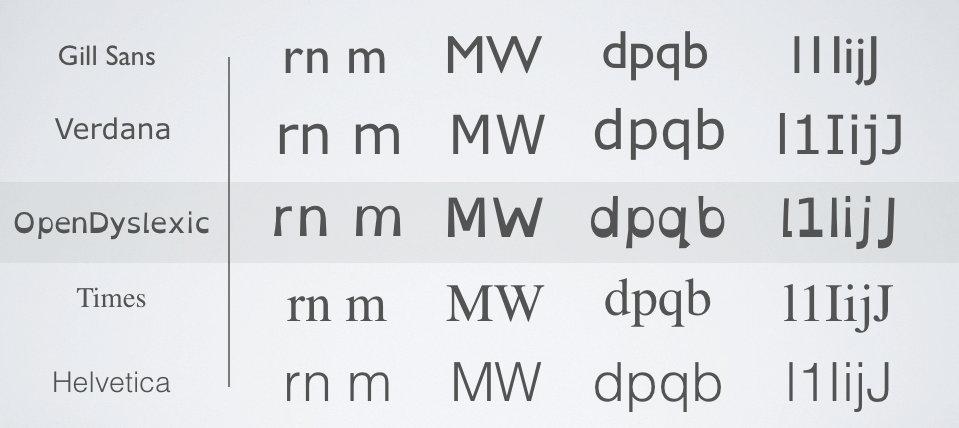
\includegraphics[width=35em]{../assets/images/open-dyslexic-abelardo-gonzalez-font-character-map.png}
                            \end{center}
                            \bigskip
                            \noindent Het is misschien een lelijk lettertype. — Althans dat vond ik in het begin. — Maar heb dit lettertype gebuikt de afgelopen maand het het leest veel fijner naar mijn mening. De eerste paar dagen moest ik echt wennen. Ik moest een soort van op nieuw leren lezen. Maar nu? Nu is het veel veel fijner. Ik gebruik extensies om dit lettertype te forceren. Dit is bijna het enige lettertype dat ik lees.
                            \bigskip
                            \noindent Een probleem dat veel mensen met dyslextie hebben is dat letters draaien en verplaatsen als je ze leest. Zoals je het in de film ziet. — though niet altijd even erg. — Als ik OpenDyslextic gebruik heb ik dit probleem niet meer. Ze blijven gewoon stil staan. Dat niet alleen, Letters lijken ook minder op elkaar.
                            \bigskip
                            \noindent Ik kan niet de enige zijn die ooit heeft opgemerkt dat van deze zes letters: \texttt{p}, \texttt{q}, \texttt{b}, \texttt{d}, \texttt{O}, \texttt{0}; het er maar twee zijn. \texttt{d} \& \texttt{O} zijn allemaal het zelfde. En dat is echt heel irritant. Zeker als je even een mindere dag hebt waar de letters op je papiertje net soep zijn. Kijk OpenDyslexic kan geen wonderen maken, maar kijk naar de afbeelding, ze hebben ze verschillend gemaakt. Dit maakt ze zo veel minder vermoeiend om te lezen.
                            \bigskip
                            \noindent Ze hebben ook funky dingen gedaan met de spacing van de letters etc. Ik kan hier uren over door gaan. Punt is, dit is een upgrade, gebruik het. Als je meer wil weten, of dit lettertype \textbf{gratis} wil downloaden, ga dan naar \underline{\hyperlink{https://opendyslexic.org/}{opendyslexic.org}.
                        }
                        \item{\textbf{Houd het visueel}. 
                            Net zoals bij de tips voor ADHD, en autisme is het belangrijk dat je dingen visueel houd. Zeker gezien lezen vaak een probleem is. Plaatjes, grafieken, en diagramen zijn een god sent.
                        }
                    \end{itemize}
        
        \subsection{Conclusion}
            Er waren een paar dingen die we hiervan kunnen leren. Een paar sterktes waar we op in kunnen spelen, en een paar zwaktes die we zouden moeten kunnen trainen en vermijden.
        
        \subsubsection{Problemen}
            Ten eerste, de meeste neurodivergente mensen zijn visueel ingeteld. Sterker nog, nadat ik mijn onderzoek heb gedaan blijkt dat 65\% visuele leerlingen zijn.\cite{Visual-Learners-are-the-most-common} Daarom moet ik zorgen dat mijn les voornamelijk visueel is ingesteld. De meeste lessen worden nu gegeven worden, worden gedaan door middel van een iemand die voor de klas staat en een verhaal verteld. Niet super ideaal. Tweede probleem is dat afhankelijk van welk type neurodivergente leerling je hebt, dat je verschillende levels van stimulatie moet hebben. Dus daar moeten we ook iets aan doen
        
        \subsubsection{Oplossingen}
            Okay sinds het meeste visueel zal moeten zullen we moeten zorgen dat dat in orde is. Een white bord zal het niet worden. Afhankelijk van wat we er op willen zetten we extreem veel tijd kwijt zijn. Als deze tijd te lang is raakt die ene ADHD'er in de hoek afgeleid. Mij zien tekenen is niet stimulerend genoeg. Dus we zullen in de voor bereiding sowieso tijd moeten stoppen in het maken van een power-point voor alle concepten die we willen behandelen. Samen met tekeningen. Het voordeel is wel. Zodra we een concept getekend hebben kunnen we deze visuele concepten recyclen. We kunnen ze namelijk ieder jaar over en over gebruiken. 
            \bigskip
            \noindent Hier is een lijst van dingen die we kunnen gebruiken om ons voorbereide powerpoint whiteboard zo appealling als mogelijk te maken voor onze visuele leerlingen.
            \begin{itemize}
                \setlength\itemsep{0em}
                \item Schrijf nieuwe vocabulary op, en kleur ze zodat ze opvallen;
                \item gebruik het whiteboard efficient. We zullen ons digitale whiteboard al van te voren gemaakt hebben
                \item Gebruik grafieken en diagrammen.
                \item Voeg symbolen en beweging toe aan flashcards.
                \item Speel flashcardspellen.
                \item Experimenteer met realia.
                \item Gebruik diavoorstellingen en video's.
                \item Moedig hen aan om vooraan te zitten.
                \item Gebruik OpenDyslextic.
            \end{itemize}
            \bigskip
            \noindent Ten tweede hoe krijgen we iedereens stimulatie levens optimaal? Ik bijvoorbeeld heb — de hele dag door — het zelfde nummer op repeat. Omdat het zelfde nummer is zit er structuur in. Bij de 5e keer weet je exact waar wat zit. Maar het is toch stimulerend. Dit werkt alleen niet voor iedereen. De ander heeft absolute stilte nodig.
            \bigskip
            \noindent Hiervoor hebben we kop telefoons. Iedereen heeft tegenwoordig kop telefoons met noice-cannelation wat betekend dat ze in stilte kunnen werken, als ze dit willen. Daarom ga ik tegen stelling tot wat andere docenten doen, het gebruik van koptelefoons stimuleren. Het houd leerlingen gefocust en afgezonderd van elkaar. Wanneer ze zelf mogen werken, werken ze dus ook alleen.
            \bigskip
            \noindent Dan hebben we nog het laatste ding. We moeten voorspelbaar zijn. Voorspelbaar en gestrucureerd. Dan weten ze precies wat ze te wachten staat. Daarom moeten we de les planning op het bord schrijven en de leerlingen uit nodigen mij als docent te verbeteren en mij aan de tijd te houden. 
        
        \subsection{Ideale les}
            Okay daar zijn we dan, een hippe 9 pagina-'s later. Laten we beginnen aan wat mijn ideale les zou zijn. Voor mijn voorbeeld neem ik een les van 50 minuten. Dit is omdat de meeste middelbare scholen lessen van 50 minuten hanteren. 
            \subsubsection{Les Inrichting}
                \paragraph{Voorbereiding}
                    We beginnen natuurlijk met de voorbereidingen. Want een goed begin is het halve werk. Plus, we hadden al eerder geconstateerd dat een goed voorbereid white board met zo veel mogelijk visuele aspecten zeer belangrijk was om de les ook visueel sterk te houden. Dus dit is waar ik zou beginnen. 
                    \bigskip
                    \noindent Allereerst moeten we een planning maken, als we deze maken kunnen we daarop verder bouwen. Het heeft geen zin als we 100 slides aan uitleg maken en maar 5 minuten er voor over houden. Dat is is een nieuwe slide elke 3 seconden. Het is belangrijk dat we onze planning SMART noteren, dit houd ons consistent, aanspreekbaar, en controleerbaar. Boven op dat het ons op schema houd, kan het zijn dat leerlingen nieuwsgierig worden. De leerlingen zijn dan onbewust actief het leer process aan het ondersteunen door hun zelf te motiveren en verwachtingen opstellen.\cite{NAME-ME}
                    \bigskip
                    \noindent Hierna zou ik beginnen met een mind-map over het onderwerp en alles wat er aan gerelateerd is. \hyperlink{https://www.mindnode.com}{\underline{Mind Note}} is een fantastische app hiervoor. De subscription is een scam, maar de gratis versie werkt fantastisch. 
                    \bigskip
                    \begin{center}
                        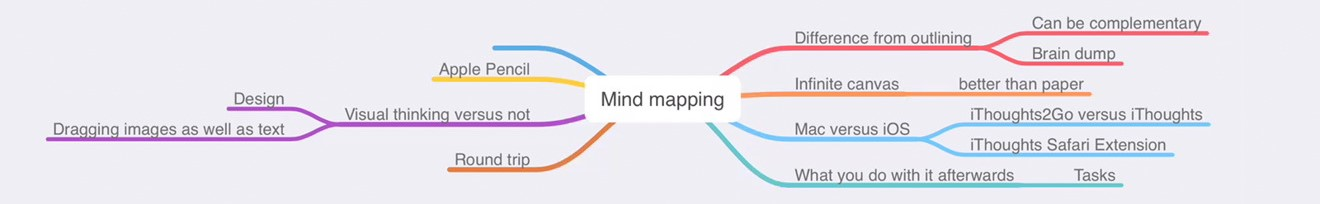
\includegraphics[width=35em]{../assets/images/mind-note.jpg}
                    \end{center}
                    \bigskip
                    \noindent Next, kunnen we beginnen aan de Dia-'s. Hierbij gebruiken we de Mind Note van eerder. Hiermee kunnen we gemakkelijk hoofdzaak van bij zaak scheiden. Nadat we dat gedaan hebben Passen we de een paar principes toe. We maken dingen dik gedrukt en gekleurd als het belangrijk is. Max een gekleurd ding op een slide. Afbeeldingen in plaats van woorden waar mogelijk. Lettertype is OpenDyslextic, uiteraard. Tot slot, een grote ergernis van mij, onderstreep het woord \underline{niet}. Ik lees zo vaak over dit woord heen, en ik weet dat een hoop dyslexten dit ook doen. Dit word is gewoon onzichtbaar, ik weet niet waarom.
                    \bigskip
                    \noindent Nu dat we ons white board, verhaal, en visuals voorbereid hebben zijn we klaar om de les te beginnen.
                \paragraph{Terug halen van de voor kennis (5 minuten)}
                    We beginnen de les met het ophalen van de voorkennis. We moeten namelijk er voor zorgen dat de kennis die nodig is voor de uitleg van straks al klaar staat. Als ze niet weten wat een driehoek is, wens ik je veel succes met het uitleggen met wat een gelijkbenige driehoek is. We willen de voorkennis activeren door middel van het stellen van vragen. Het is belangrijk dat we positief blijven, en ons "samen" opstellen\cite{samen-boven-leads-to-better-results}. We willen ze niet afschrikken, of laten voelen alsof we ze aan het overhoren zijn. Het moet een soort van spel zijn. Dit helpt vooral mensen met ADHD. Mensen met ADHD leren veel sneller in spel vorm.\cite{ADHD-en-games}
                    Zodra een leerling antwoord geeft zijn d'r drie dingen die d'r kunnen gebeuren.
                    \begin{itemize}
                        \item{\textbf{Een, de leerling heeft het goed.}
                            Zodra een vraag goed is beantwoord herhalen we dit. Dit is belangrijk omdat het kan zijn dat er leerlingen afgeleid waren, of het oprecht niet hadden gehoord. Door middel van het goede antwoord te herhalen zorgen we d'r voor dat de leerlingen nóg een keer over heen gaan. We voegen er daarnaast ook een compliment aan toe. We willen ze belonen voor hun nek uit te steken. En we willen natuurlijk dit gedrag stimuleren. 
                        }
                        \item{\textbf{De leerling heeft de vraag half goed.}
                            We starten natuurlijk met het juiste te herhalen. Het foute herhalen we niet. Het juiste moet namelijk in hun hoofd blijven zitten. Daarna geven we een compliment omdat we dit het antwoord geven willen stimuleren. We vragen aan de klas of iemand anders kan helpen. Het is belangrijk dat we niet vragen of iemand anders het wel weet. Want dan zeggen we indirect dat de eerste leerling het fout had, en dat hadden we 'niet gehoord'. We vragen het alsof we samen een puzzel aan het oplossen zijn, en hulp nodig hebben. Dit houd de gedachte er in dat het een spelletje is. Daardoor ligt er geen druk op de leerlingen om het juist te hebben.\cite{games-help} En helpt het studenten leren door middel van trial-en-error.\cite{games-help}
                        }
                        \item{\textbf{De leerling zit d'r compleet naast.}
                            We beginnen met het zeggen waarom dit niet klopt en een hint naar het juiste antwoord. Daarna geven we natuurlijk een compliment. We vragen wederom of een student ons kan helpen met deze puzzel. Het is belangrijk positief te blijven.
                        }
                    \end{itemize}
                    \bigskip
                    \noindent De rede dat we de voorkennis herhalen is omdat het vaak opbrengen van iets lijd tot dat dat ding opgeslagen word in het lange termijn geheugen.\cite{repeating-leads-to-long-term-memory} Dus door het activeren van de voorkennis zorgen we er voor dat de les stof in het langer termijn geheugen komt. Precies waar we het willen hebben.
                \paragraph{Uitleg (5 minuten + 5 in bruikleen)}
                    Nu dat we de voorkennis herhaald hebben is het belangrijk dat we hier op verder bouwen. We beginnen met duidelijk het les doel te herhalen. Het is namelijk belangrijk dat we de leerlingen activeren voor het belangrijkste stukje van de les. We vragen de leerlingen of ze dit concept al snappen, of zouden kunnen uitleggen. 
                    \bigskip
                    \noindent Als een leerling een poging maakt geven we die een compliment en herhalen we het goede dat nog niet te ver is van de voorkennis. Als een leerling het helemaal goed uitlegde en het concept begreep geven we hem een zakje snoep. Waarom doen we dit? Nou, zoals ik al eerder zei, de les een een spelletje. En wat gebeurd er als je de jackpot scored op een game show? Dat klopt, dan krijg je een flinke beloning. 
                    \bigskip
                    \noindent Helaas kan ik geen 10 euro weg geven iedere keer, want zoveel krijg je als leraar niet betaald. Gelukkig hoeft dat ook niet. Een zakje snoep is een veel grotere beloning dan een compliment. Suiker geeft een grote lading dopamine vrij vergelijkbaar met drugs.\cite{sugar-equals-drugs} Ik ben geen voorstander om kinderen drugs te voeren. Maar dit ziet er veel belovend uit. Niet allen stimuleert het om complexe vraagstukken zelf al proberen op te lossen, het stimuleert leerlingen om zelf studie te doen en in het voren te werken. Ze weten namelijk dit onderwerp de volgende les behandeld word en dat dit studeren beloond word. 
                    \bigskip
                    \noindent Ongeacht wat de leerlingen antwoorden, leggen het concept uit. Maar afhankelijk van hoeveel leerlingen de vraag wilde/dacht te kunnen antwoorden krijgen we een schatting van hoeveel tijd leerlingen nodig hebben voor dit concept. Als niemand ook maar een poging kon maken is het duidelijk dat dit concept meer tijd nodig heeft. Dan nemen we de volle 10 minuten. Als iedereen het eigenlijk al wist dan hebben we maar 5 minuten nodig en kunnen we deze gebruiken in de vragen ronden. 
                    \bigskip
                    \noindent Mijn uitleg zal veel voorbeeld vragen bevatten. Waarom doe ik dit zo? Theorie is cool en al, maar zo leer je niet altijd. Nadat het concept is uitgelegd leg ik oppervlakkig de theorie uit. Leerlingen die de diepere theorie er achter willen weten happen toch wel. Die vragen dadelijk privé hoe het diepere stuk er uit zit. Wat doen we als ze zulke goede vragen stellen en graag in het diepere, moeilijkere stuk willen werken? That's right, jackpot, zakje Haribo voor de gelukkige. Dit willen we stimuleren en herbergen. Nieuwsgierigheid en enthousiasme. Dit geld ook voor leerlingen die het na de uitleg nog niet snapte en vroegen om extra uitleg. Dat is goed gedrag. We geven ze een complimentje, en zeggen dat ze het heel goed gedaan hebben. Daarna melden we de we volgende les terug komen en checken of de leerling het nog steeds snapt. Doen ze dit? Extra complimentje. Door er op terug te komen herhalen we het nog een keertje met de leerling en zorgen we er voor dat we gegarandeerd het juiste concept in het langer termijn geheugen van de leerling proppen.
                \paragraph{Instructie (10 minuten)}
                    We beginnen de instructie met uitleggen wat het doel is van de instructie, en welke opdrachten we af gaan maken. Dan weten de leerlingen waar ze aan toe zijn en wat van ze verwacht wordt. Het doel van de instructie is dat ze inzien wat ze moeten doen om de stof die ze zojuist hebben geleerd to te passen. Daarom maken we ze de opdrachten eerst samen in de instructie. Zo heeft iedere leerling de kans om te zien hoe je met deze stof werkt.
                    \bigskip
                    \noindent Een probleem dat veel voorkomt is dat de stof te snel word uitgelegd wanneer het lastig word. Daarom pas ik een automatische strategie toe waarbij ik persoonlijk geen moeite hoef te steken om het werkende te houden en niet alleen leerlingen het tempo bepalen maar ook zorgen dat de stof gegarandeerd duidelijk is. Dit doe ik door duidelijk te maken dat door vragen te stellen je me vertraagd. Dan hebben hun niet alleen de tijd om te begrijpen wat er gebeurd, maar ook de kans om te zorgen dat ze het snappen. Ik heb dit in de praktijk gezien door meerdere leraren, die dit met 100\% succes rate toepasten.\cite{succesfull-instructions} Zodra de leerlingen door hebben dat vragen stellen beter werkt dan het maar snel op te schrijven om er later op terug te komen.
                    \bigskip
                    \noindent Iets heel belangrijks dat we moeten doen als we de instructie doen is het zorgen dat we elke keer andere studenten pakken. Als we dit niet doen krijg je dat die ene slimme student alle antwoorden geeft. 
                \paragraph{Groepsopdracht (10 minuten)}
                    Deze vraag is moeilijker dan de vragen die ik zojuist met ze gemaakt heb en word gemaakt in paren en anders alleen. Dit is omdat je al snel krijgt dat twee het werk doen en de derde er bij zit. Als je het met z'n tweeën doet, heb je dat probleem niet. Als bonus heb je dat dit voor mensen die sociaal niet zo sterk zijn het nu makkelijker is om te oefenen. Success om tussen twee mensen te komen als je dit dood eng vind, niet sociaal bent, en niet eens zeker weet of je ideee wel goed is. Terwijl het voorstellen van een idee aan één persoon die verwacht dat jij ook input leverd en boom! Dat is een veel beter idee. Het helpt ook met mensen met autisme. Zei zijn vaak de minder sterke op een sociaal vlak. Ergens hierboven 5 pagina's terug had ik beschreven bij de autisme les-tips dat een-op-een opdrachten een hele goede oefening zijn voor mensen met autisme om te oefenen op sociaal vlak. Gezien zei vaak beter zijn in technische vakken verwacht ik dat de ander weet dat deze hiervan veel kan leren en zich vooral naar de gene met autisme zal kijken. Waardoor de gene met autisme een goede kans heeft om uit te leggen en te oefenen met zijn sociale skills. Ik vind het daarom ook totaal niet erg dat leerlingen niet onderling over niet stof gerelateerde dingen praten. Dit gaan ze namelijk toch wel doen. Zo kan ik zorgen dat de concentratie tank weer vol loopt terwijl ze ook bezig zijn met de stof.
                    \bigskip
                    \noindent Nadat de 5 minuten aan werken aan de opdracht, plus 5 minuten van leerlingen die met elkaar praten over zijn, gaan we de opdracht bespreken. Dit doen we weer samen klassicaal. Dit doen we alleen later. Eerst vraag ik alle leerlingen om hun antwoorden in te  leveren. Deze kijk ik na voor de meest gemaakte fouten. Deze behandel ik later.
                    \bigskip
                    \noindent De opdracht die ze maken is een van de opdrachten die ik voor ze heb uitgekozen. Ik zou meerdere opdrachten uitkiezen die ze zouden kunnen maken en ze dan zelf laten kiezen. Omdat ze zelf mogen kiezen welke ze maken ontstaat er intrinsieke motivatie.\cite{NAME-ME} Dat zal leerlingen motiveren om de groepsopdracht te maken. Bovenop beloon ik ieder tweetal dat meer dan een opdracht maakt. Het vertonen van meer doen dat dat van je gevraagd word, word uiteraard beloond.
                \paragraph{Zelfstandig werken (10 minuten)}
                    Ik geef ze 10 minuten om aan huiswerk te werken. Dit geeft mij de tijd om de groepsopdracht na te kijken. Vaak vinden leerlingen dit fijn omdat ze dan minder thuis hoeven te doen. Dit vergroot ook de kans dat ze het huiswerk thuis ook daadwerkelijk maken omdat er minder nog gedaan moet worden.\cite{more-homework-equals-bad} Dit helpt ook met het verminderen van de kans op ene amygdala-kaping.\cite{more-homework-equals-bad} 
                    \bigskip
                    \noindent Zoals ik al eerder had vermeld geef ik hier leerlingen de kans om hun koptelefoons te gebruiken. Dit geeft mensen met autisme die zich nu misschien moe voelen na deze grote hoeveelheid verplichte interacties met mede studenten de kans om van al deze prikkels bij te komen. Het geeft de mensen met ADHD een kans om hun concentratie bij te tanken door middel van alle stimulatie die de kop telefoon geeft. Bovendien zorgt het er voor dat de tank niet leeg loopt. Als je iemand met ADHD in een muis stille kamer neer zet waar die alleen moet werken zonder enige stimulatie gaat deze onrust veroorzaken. Daar kunnen mensen met ADHD niks aan doen, ze hebben gewoon stimulatie nodig. Door koptelefoons te gebruiken laten ze ook mede studenten met rust. Bovendien ervaren leerlingen het mogen luisteren naar muziek als belonen, waardoor ik meer "samen" uitstraal. Wat zorgt voor betere prestaties.\cite{samen-boven-leads-to-better-results}
                \paragraph{Bespreken meest gemaakte Fouten tijdens Groepsopdracht (5 minuten)}
                    Nadat ik door de oplossingen van de groepsopdracht ben heen gegaan ben, heb ik een idee met wat de leelingen het meeste struggelen. Ik ga dan samen met ze de opdracht maken. Eerst bereid ik mijn white board voor door midddel van de opdracht zelf uit te werken tot en met de fout die het meeste gemaakt is. Dan maak een dia met de fout gekleurd zodat het duidelijk is dat dit speciaal is. Ik vraag de leerlingen dan wat hier niet klopt, en wat we anders kunnen doen. Dan ga ik naar de volgende dia waar de foute stap vervangen is door de goede. Nog steeds opvallend gemarkeerd. Hierdoor onthouden leerlingen deze veel gemaakte fout beter.\cite{Visual-Learners-are-the-most-common} De gene die deze fouten gemaakt hadden voelen zich wel aangesproken omdat ze weten dat het om hun fout gaat, maar omdat ze anoniem blijven is er geen kans dat er schaamte ontstaat. Dit voorkomt een amygdala-kaping, of een shutdown.\cite{more-homework-equals-bad}\cite{autisme-shutdowns} Omdat de leerlingen aan het reflecteren zijn of zij deze fout gemaakt hadden en of ze begrijpen hoe het wel moet vind een meta cognitieve leer activiteit plaats.\cite{NAME-ME}
                \paragraph{reflectie (5 minuten)}
                    Als er tijd over is omdat de uitleg geen 10 minuten hoeft te zijn. Is er tijd over voor reflectie. Hier geven we de leerlingen een complimentje over wat ze deze keer goed gedaan hebben. Ik ben persoonlijk niet van de vlakke complimentjes zoals "Goed gewerkt vandaag!" omdat dit onpersoonlijk is, en fake aanvoelt. Ik zou mijn complimentje persoonlijker maken zoals dat ik het heel fijn vond hoe goed ze de instructie hadden mee gedaan. Niet alleen is een persoonlijker complimentje echter. Het helpt ook met het aanmaken van zelf vertrouwen van de leerling.\cite{compliments-how-to}
            \subsubsection{Waarom dit een goede les in richting is}
                Mijn ideale les bestaat uit een sterkte afwisseling van leertheorieen en leeractiviteiten. Dit houd de leerlingen scherp en zorgt dat de leerlingen en zorgt dat de leerlingen hun concentratie tot de max kunnen gebruiken. Daar boven op wissel ik constant hoe de leerling zich moet opstellen tussen een passieve en een actieve houding. Ik vind dat de leerlingen veel vrijheid, complimenten, en stimulatie om verder te gaan krijgen wat in mijn optiek zorgt voor een goede leer omgeving waar de leerling de kans krijgt om op hun eigen tempo ver te gaan. Ik zou zegen dat ik tijdens de hele les ”samen-boven” uit straal. Wat voor leerlingen de ideale opstelling was.\cite{samen-boven-leads-to-better-results} Bovenop zorg ik voor strucuur en ondersteuning.
            \subsubsection{Waarom dit ook goed werkt voor neurodivergente leerlingen}
                Over ondersteuning gesproken, hoe heb ik de neurodivergente leerlingen ondersteund? Dat was namelijk het hele doel van dit passie projectje. Ik zou zeggen dat ik dit goed gedaan heb. Ik bood visuele ondersteuning. Hield structuur en mezelf voorspelbaar. Bood voor 60\% van de les de tijd voor leerlingen om te vragen stellen. Gaf neurodivergente leerlingen een kans om in een veilige omgeving te werken aan hun zwakke punten. En tot slot speelde in op hun sterke punten. Hoewel ik geen PhD heb in hoe je neurodivergente leerlingen moet les geven vind ik dat dit een geslaagde zelf verzonnen bonus objectieve is en ben ik trots op de aanpassingen die ik heb gemaakt in vergelijking met de lessen die ik altijd heb gekregen.

    %| ------------------------------------------------------------------------------------------------------------- |%
    %|                                           Beeld van den Leerlingen                                            |%
    %| ------------------------------------------------------------------------------------------------------------- |%
    
    \section{Beeld van de Leelingen}
        \textbf{Beeld van leerlingen. Stel je voor dat je leerlingen hoort praten over jou als docent. Wat zou je willen dat ze dan zeggen? Wat zou je zeker niet willen dat ze zeggen? Waarom?}
        \subsection{Wat ik hoop dat ze zeggen}
            Er is een ding waar ik oprecht heel blij van zou worden. Als mijn leerlingen zouden zeggen dat ze enthousist worden van mij. Dat ze het leuk vinden om naar mijn lessen te komen. Niet alleen zou dit betekenen dat leerlingen open staan voor mij en mijn lessen, maar ook dat het leerprocess met mij oprecht leuk is. 
            \bigskip
            \noindent In een van de lessen was er een hele goede Engels docent. — Ik ben zijn naam vergeten. — Toen zijn filmpje begon had ik de gedachte van "Ha engels litratuur docent, dat is nou iets wat ik echt niet zou willen worden. Ik snap het nut daar dus echt niet van." Maar ik kan met alle zekerheid zeggen dat ik daar fout zat. 
            \bigskip
            \noindent In het filmpje was hij aan het les geven op een manier die mij zo aansprak. Die docent was aan het voorlezen. Maar je kon het verhaal echt voor je zien. Maar het was oprecht zo leuk om te zoien. Hij leefde echt in het verhaal, je kon de passie zien zeg maar. Dat sprak mij aan. Ik \hyperlink{https://en.wikipedia.org/wiki/Dungeon_Master}{\underline{DM}} voor de lol, en mijn taak daar is om dan aan een groep spelers de situatie te scheten, en een goed verhaal te vertelen waarin zij de hoofdrol spelen. Dus de hoeveelheid passie waarmee hij zijn verhalen vertelde raakte me.
        \subsection{Wat ik absolute hoop dat ze niet zeggen}
            Ik zou echt het laatste zou zijn dat ik van ze zou willen horen is dat mijn leerlingen denken dat mijn lessen geen waarde toevoegen aan hun leerproces en dat ze er echt niet heel willen. Ik vind het echt super belangrijk dat ze zich betrokken voelen en de lesstof begrijpen. Als leerlingen weg willen van mij en mijn lessen zou ik dat echt heel pijnlijk vinden. Ik denk ook niet dat als dat de sfeer is dat ik mijn leerlingen iets geleerd krijg, omdat zij dan niet open staan om bij mij en mijn lessen te zijn. En omdat ik dan niet de zelfde engerie uit kan stralen als ik weet dat het ongewenst is.
    \newpage

    %| ------------------------------------------------------------------------------------------------------------- |%
    %|                                                  Disclaimer                                                   |%
    %| ------------------------------------------------------------------------------------------------------------- |%
    
    \section{Disclaimer}
        Ik wil wel effe de disclaimer gemaakt hebben dat voor iedere ADHD'er, autist, Dyslext, Queer, of welke groep dan ook, we allemaal individuen zijn. Ik heb gesproken voor de groep vanuit mijn ervaringen maar ieder persoon is anders. Hoewel wel vergelijkbare zwakke of sterke punten hebben wil dat niet zeggen dat we allemaal het zelfde zijn. Wat voor mij werkt, werkt misschien niet voor iemand anders. Als jij of iemand die je kent vragen hebt, spreek dan met een professional, en misschien nog wel belangrijker het individu er achter.
    
    %| ------------------------------------------------------------------------------------------------------------- |%
    %|                                                   Nawoord                                                     |%
    %| ------------------------------------------------------------------------------------------------------------- |%
    
    \section{Nawoord}
        Ik merk dat zelfs ik een hoop informatie mis en niet zo veel weet over zowel mijn eigen condities als die van andere. Dus ik kan zeker in zien hoe iemand die in hun persoonlijke leven niet veel te maken heeft ment neurodivergente mensen ook een hoop niet wist. 
        \bigskip
        \noindent Ik weet en merk dat er veel vooroordelen zijn voor neurodivergente mensen. Zoals dat ADHD'ers lui zijn of mensen met autisme geen/weinig empathy hebben. En ik hoop dat men in de toekomst meer kan werken aan het weg werken van dit soort opvattingen. 
        \bigskip
        \noindent Artistic-Liberty is hoe ik mijn invulling voor deze opdracht zou noemen. Zal de opdracht wel niet helemaal heb gedaan zoals dat men misschien van mij verwachte. Maar in de alle lessen die we gedaan hebben in dit kwartaal, hoe veel gingen er over vormen van neurodiversiteit? Hoe je hier mee om moet gaan? Hoe je dit kan ondersteunen? Nul. Like oprecht, geen een les ging over hoe je deze soort, mijn soort, goed kan ondersteunen. En ik vind dit een gemiste kans. Ik denk dat er echt wel een week besteed kan worden. Dan heb ik het niet over de volle week. Maar een bijgevoegd filmpje bij de voorbereiding moet kunnen.
        \bigskip
        \noindent Ik wist niet precies wat ik met dit passion project wou bereiken toen ik er aan begon. Het leek me een goede manier om op een andere creatieve manier dit essay te schrijven. Maar wat ik achteraf nu zou willen is dat het onderwijs soms wat meer afgesteld werd voor mij en mensen zoals mij. Ik weet niet alleen uit persoonlijke ervaring dat dit kan. Ik weet  dat het werkt. 
        \bigskip\bigskip
        — Tygo
        \label{LastPage}
    \newpage
    
    %| ------------------------------------------------------------------------------------------------------------- |%
    %|                                                Litratuur lijst                                                |%
    %| ------------------------------------------------------------------------------------------------------------- |%
    
    \bibliographystyle{IEEEtran}
    \pagestyle{empty}
    \renewcommand{\refname}{Literatuurlijst}
    \begin{thebibliography}{9}

        \item[\bigskip\subsection*{Neurotypisch}]
            \bibitem{enthusiasm-creates-motivation}
                Deci, R. R. E. (2000). Self-determination theory and the facilitation of intrinsic motivation social development, and well-being. Geraadpleegd op 25 Oktober 2023, van \url{https://selfdeterminationtheory.org/SDT/documents/2000 RyanDeci SDT.pdf}.
            \bibitem{intrinsic-motivation-is-more-important}
                Goes, L. (2009). De invloed van intrinsieke- en extrinsieke motivatie op schoolprestaties Geraadpleegd op 25 Oktober 2023, van \url{https://studenttheses.uu.nl/bitstream/handle/20.500.12932/4563/0443603%20LCM.Goes.pdf?sequence=1}.
            \bibitem{extrinsic-motivation-results-in-supperfical-learning}
                Leren, V. (n.d.). Leidt verhoogde motivatie tot betere leerresultaten? Geraadpleegd op 25 Oktober 2023, van \url{https://www.voortgezetleren.nl/leidt-verhoogde-motivatie-tot-betere-leerresultaten/}.
            \bibitem{samen-boven-leads-to-better-results}
                den Brok, P. (2011). Interpersoonlijke ontwikkeling van de docent. Geraadpleegd op 25 Oktober 2023, van \url{https://www.scribd.com/document/341217615/Reader-Interpersoonlijk-Den-Brok}
            \bibitem{repeating-leads-to-long-term-memory}
                Gretchen Schmelzer. (11 Januarie 2015). Understanding Learning and Memory: The Neuroscience of Repetition. Geraadpleegd op 23 Oktober 2023, van \url{https://gretchenschmelzer.com/blog-1/2015/1/11/understanding-learning-and-memory-the-neuroscience-of-repetition}
            \bibitem{NAME-ME}
                Vermunt. J.D. (juni 1999). Congruence and friction between learning and teaching. Geraadpleegd op 25 Oktober 2023, van \url{https://www.sciencedirect.com/science/article/abs/pii/S0959475298000280}
            \bibitem{Kids-that-dont-emtion-perform-worse}
                Bart L.J. Looman, Marlies de Jager, Bram Tuk, Simone A. Onrust, Jeroen Lammers, Marion Spijkerman, Goof Buijs. Sociaal-emotionele ontwikkeling in het primair onderwijs: Een doorlopende integrale aanpak? Geraadpleegd op 23 Oktober 2023, van \url{https://www.kennisrotonde.nl/sites/kennisrotonde/files/migrate/291-antwoord-lestijd-vo.pdf}
            \bibitem{games-help}
                DigitalCitizenship. Teaching and learning with games. Geraadpleegd op 23 Oktober 2023, van \url{https://www.digitalcitizenship.nsw.edu.au/articles/teaching-and-learning-with-games}
            \bibitem{more-homework-equals-bad}
                CLIFTON PARKER. B. (10 Maart 2014). Stanford research shows pitfalls of homework. Geraadpleegd op 24 Oktober 2023, van \url{https://news.stanford.edu/2014/03/10/too-much-homework-031014/}
            \bibitem{compliments-how-to}  
                Tremio, K. (13 januari 2017). Effectieve complimenten geven: Hoe doe je dat? Geraadpleegd op 23 Oktober 2023, van \url{https://www.onderwijsvanmorgen.nl/effectieve-complimenten-geven-hoe/}
        \newpage

        \item[\bigskip\subsection*{ADHD}]
            \bibitem{ADHD-behoeftes}
                NHS. (24 December 2021). Living with Attention deficit hyperactivity disorder (ADHD). Geraadpleegd op 25 Oktober 2023, van \url{https://www.nhs.uk/conditions/attention-deficit-hyperactivity-disorder-adhd/living-with/}.
            \bibitem{ADHD-video-working-memory}
                How to ADHD. (22 Juni 2021). Why I Can't Remember Things -- How ADHD Affects Working Memory. Geraadpleegd op 25 Oktober 2023, van \url{https://www.youtube.com/watch?v=HszXKZO_H18&ab_channel=HowtoADHD}.
            \bibitem{ADHD-video-prioriteiten}
                How to ADHD. (28 September 2023). How ADHD Affects Prioritization (And Why Recognizing IBNUs Can Help). Geraadpleegd op 25 Oktober 2023, van \url{https://www.youtube.com/watch?v=5xbD9t8cM4M}.
            \bibitem{ADHD-video-rejection-sensitivity}
                Kati Morton. (21 Jun 2021). What is Rejection Sensitive Dysphoria? Geraadpleegd op 25 Oktober 2023, van \url{https://www.youtube.com/watch?v=ZQ44ynEjsHQ&ab_channel=KatiMorton}.
            \bibitem{ADHD-rejection-sensitivity}
                Cleveland Clinic. (30 Augustus 2022). Rejection Sensitive Dysphoria (RSD). Geraadpleegd op 25 Oktober 2023, van \url{https://my.clevelandclinic.org/health/diseases/24099-rejection-sensitive-dysphoria-rsd}
            \bibitem{ADHD-resilience}
                Sydni Rubio, Hannah Riley, Sina Eißfeller. (10 mei 2022). The gift of resilience: Why ADHD makes us stronger. Geraadpleegd op 26 Oktober 2023, van \url{https://www.getinflow.io/post/adhd-gift-resilience-makes-us-stronger}
            \bibitem{ADHD-creativity}
                Zahavit Paz. Is the ADHD Brain More Creative? Geraadpleegd op 24 Oktober 2023, van \url{https://www.ldrfa.org/does-adhd-enhance-creative-abilities}
            \bibitem{ADHD-visual}
                Bette Fetter. (8 Maart 2021). See It, Learn It: Make Homework Come Alive for Visual Learners. Geraadpleegd op 24 Oktober 2023, van \url{https://www.additudemag.com/visual-learner-homework-help}
            \bibitem{ADHD-classroom}
                CDC. (27 September 2023). ADHD in the Classroom: Helping Children Succeed in School. Geraadpleegd op 24 Oktober 2023, van \url{https://www.cdc.gov/ncbddd/adhd/school-success.html}
            \bibitem{ADHD-Neurobiologie}
                Wikipedia. (12 Augustus 2023). ADHD. Geraadpleegd op 24 Oktober 2023, van \url{https://nl.wikipedia.org/wiki/ADHD#Neurobiologie}.
            \bibitem{ADHD-Bijkomende-problematiek}
                Wikipedia. (12 Augustus 2023). ADHD. Geraadpleegd op 24 Oktober 2023, van \url{https://nl.wikipedia.org/wiki/ADHD#Bijkomende_problematiek}.
            \bibitem{ADHD-Behandeling}
                Wikipedia. (12 Augustus 2023). ADHD. Geraadpleegd op 24 Oktober 2023, van \url{https://nl.wikipedia.org/wiki/ADHD#Behandeling}.
            \bibitem{ADHD-Niet-medicinale_behandelingen}
                Wikipedia. (12 Augustus 2023). ADHD. Geraadpleegd op 24 Oktober 2023, van \url{https://nl.wikipedia.org/wiki/ADHD#Niet-medicinale_behandelingen}.
            \bibitem{ADHD-en-games}
                Wikipedia. (12 Augustus 2023). ADHD. Geraadpleegd op 24 Oktober 2023, van \url{https://nl.wikipedia.org/wiki/ADHD#Serious_games}.
            \bibitem{ADHD-en-autismespectrumstoornissen}
                Wikipedia. (12 Augustus 2023). ADHD. Geraadpleegd op 24 Oktober 2023, van \url{https://nl.wikipedia.org/wiki/ADHD#ADHD_en_autismespectrumstoornissen}.
        \newpage     

        \item[\bigskip\subsection*{Autisme}]
            \bibitem{Autisme}
                Wikipedia. (27 okt 2023). Autisme. Geraadpleegd op 27 Oktober 2023, van \url{https://nl.wikipedia.org/wiki/Autisme}.
            \bibitem{Autisme-lesgeven}
                WaterFord. (10 Maart 2021). 30 Activities, Teaching Strategies, and Resources for Teaching Children with Autism. Geraadpleegd op 27 Oktober 2023, van \url{https://www.waterford.org/education/15-activities-teaching-strategies-and-resources-for-teaching-children-with-autism/}.
                \bibitem{ADHD-en-autisme-overlap}
                Camille Hours, Christophe Recasens, Jean-Marc Baleyte. (28 Februari 2022). ASD and ADHD Comorbidity: What Are We Talking About? Geraadpleegd op 27 Oktober 2023, van \url{https://www.ncbi.nlm.nih.gov/pmc/articles/PMC8918663/}
                \bibitem{autisme-shutdowns}
                Luke Aylward. What are autistic shutdowns and why do they happen? Geraadpleegd op 27 Oktober 2023, van \url{https://www.bristolautismsupport.org/autism-autistic-shutdowns/}
            \bibitem{autisme-upsides} 
                Blossom Childrens Center. (25 April 2023). 7 Incredible Benefits of Autism for Autistic Children. Geraadpleegd op 27 Oktober 2023, van \url{https://blossomchildrenscenter.com/2023/04/25/7-incredible-benefits-of-autism-for-autistic-children/}
            \bibitem{autisme-teaching-them} 
                Positive Action Staf. (25 September 2023). 10 Effective Tips for Teaching Children With Autism in 2023. Geraadpleegd op 27 Oktober 2023, van \url{https://www.positiveaction.net/blog/tips-for-teaching-autistic-children}
            \bibitem{autisme-visual} 
                Lisa Jo Rudy. (25 Oktober 2023). Visual Thinking and Autism: How Visual Tools Can Help Autistic People to Learn and Thrive. Geraadpleegd op 27 Oktober 2023, van \url{https://www.verywellhealth.com/visual-thinking-and-autism-5119992}

        \item[\bigskip\subsection*{Neurodivergent (algemeen)}]
            \bibitem{neurodivergent}
                via \url{https://my.clevelandclinic.org/health/symptoms/23154-neurodivergent} gebruik ik voor de onderbouwing dat er mensen bestaan met een van de grond op anders opgebouwd brein.
            \bibitem{neurodivergent-types}
                \url{https://www.forbes.com/health/mind/what-is-neurodivergent/}
            \bibitem{UDL-guidelines}
                \url{https://udlguidelines.cast.org/}
        \newpage        

        \item[\bigskip\subsection*{Dyslextia}]
            \bibitem{Dyslextie-breinen}
                via \url{https://medium.com/the-ascent/on-the-dyslexic-mind-f6ddb43915d} werd uitgelegd hoe mensen met dyslextie andere breinen hebben die informatie anders verwerken. Citaat: "Because the dyslexic mind is wired in a slightly different way than non-dyslexic minds, we process information differently. This makes us really good at some things but it also means we may struggle with other things, especially if the learning process is not adapted to our way of thinking."    
            \bibitem{dyslextia-struggles-and-superpowers}
                Margo. Things Dyslexia Students Struggle With And Their Hidden Superpowers.  Geraadpleegd op 27 Oktober 2023, van \url{https://oxfordspecialisttutors.com/things-dyslexia-students-struggle-with/}
            \bibitem{dyslextia-different-types-of-memory}
                Root. (14 Mei 2022). Why Some Dyslexics Have Trouble Following Instructions. Geraadpleegd op 27 Oktober 2023, van \url{https://www.learningsuccessblog.com/blog/dyslexia/why-some-dyslexics-have-trouble-following-instructions}
            \bibitem{Creativity-and-Dyslexia}
                Marie Lunney. (16 December 2016). Creativity and Dyslexia. Geraadpleegd op 28 Oktober 2023, van \url{https://www.lexercise.com/blog/creativity-and-dyslexia}

        \item[\bigskip\subsection*{Queerness}]
            \bibitem{LGBT-vs-CISHET-breinen}
                Mikhail Votinov, Katharina S. Goerlich, Andrei A. Puiu, Elke Smith, Thomas Nickl-Jockschat, Birgit Derntl, Ute Habel. (3 Maart 2021). Brain structure changes associated with sexual orientation. Geraadpleegd op 27 Oktober 2023, van \url{https://www.nature.com/articles/s41598-021-84496-z}.

        \item[\bigskip\subsection*{Overig}]
            \bibitem{most-important-brain-dev-age}
                First Things First. Brain Development. \url{https://www.firstthingsfirst.org/early-childhood-matters/brain-development/}
            \bibitem{hyperfocus}
                Smitha Bhandari, Stephanie Langmaid. (25 Augusts 2022). Hyperfocus. Geraadpleegd op 27 Oktober 2023, van \url{https://www.webmd.com/add-adhd/hyperfocus-flow}
            \bibitem{Visual-Learners-are-the-most-common}
                Parker. Understanding Different Types of Learning Styles. Geraadpleegd op 27 Oktober 2023, van \url{https://sites.google.com/a/litchfieldschools.org/parker-lhs-lc-9-12/home/understanding-different-types-of-learning-styles}
            \bibitem{1-in-10-pygy}
                CBS. (25 November 2019). Waardering voor zorgverleners. Geraadpleegd op 20 Oktober 2023, van \url{https://www.cbs.nl/nl-nl/longread/statistische-trends/2019/waardering-voor-zorgverleners/1-inleiding}
            \bibitem{social-isolation-affect-a-childs-mental-health-and-development}
                How does social isolation affect a child’s mental health and development? Geraadpleegd op 20 Oktober 2023, van \url{https://www.noisolation.com/research/how-does-social-isolation-affect-a-childs-mental-health-and-development}
            \bibitem{sugar-equals-drugs}
                Sugar and Dopamine: The Link Between Sweets and Addiction. Geraadpleegd op 22 Oktober 2023, van \url{https://wellnessretreatrecovery.com/sugar-and-dopamine-link-sweets-addiction/}
            \bibitem{succesfull-instructions}
                K. Veroy-Grepl. (2023). Successfull instructions. \url{https://www.tue.nl/en/research/researchers/karen-veroy-grepl}
    \end{thebibliography}

    %| ------------------------------------------------------------------------------------------------------------- |%

\end{document}
